\documentclass{article}

\usepackage{arxiv}

\usepackage[utf8]{inputenc}
\usepackage[T1]{fontenc}
\usepackage{hyperref}
\usepackage{url}
\usepackage{booktabs}
\usepackage{amsmath,amssymb,amsfonts}
\usepackage{microtype}
\usepackage{graphicx}
\usepackage[numbers,sort&compress]{natbib}
\usepackage{algorithm}
\usepackage{algpseudocode}
\usepackage{enumitem}
\usepackage{caption}
\usepackage{cleveref}
\usepackage{tikz}
\usetikzlibrary{arrows.meta,positioning,fit,calc}

\graphicspath{{../figures/}{figures/}}
\captionsetup{font=small,labelfont=bf,skip=3pt}
\setlist{itemsep=1pt,topsep=2pt,parsep=0pt}
\setlength{\textfloatsep}{8pt plus 2pt minus 2pt}
\setlength{\floatsep}{6pt plus 2pt minus 2pt}
\setlength{\intextsep}{6pt plus 2pt minus 2pt}
\renewcommand{\topfraction}{0.9}
\renewcommand{\bottomfraction}{0.8}
\renewcommand{\textfraction}{0.1}
\renewcommand{\floatpagefraction}{0.85}
\setcounter{topnumber}{3}
\setcounter{bottomnumber}{2}
\setcounter{totalnumber}{5}
\renewcommand{\bibfont}{\small}
\setlength{\bibsep}{1.5pt}
\renewcommand{\headeright}{CS329 Course Project}
\renewcommand{\undertitle}{CS329 Foundations of AI: Multi-Agent Systems --- Course Project Report}
\renewcommand{\shorttitle}{Decentralized Help-Seeking under Changing Reliability}

\newcommand{\Uself}{U^{\mathrm{self}}}
\newcommand{\ci}[2]{#1\,{\scriptsize$\pm$\,#2}}

\title{Learning Whether, When, and Whom to Ask for Help\\in a Decentralized Multi-Agent Team\\under Changing Teammate Reliability}

\author{
  Cherukuri Harshith Sai \\ 24110091 \And
  Atragada Venkata Naga Sai Ganesh \\ 24110060 \And
  Ambati Chaitanya Ram \\ 24110035 \And
  Dasari Lohith \\ 24110100 \AND
  Indian Institute of Technology Gandhinagar
}
\date{}

\begin{document}
\maketitle

\begin{abstract}
An agent in a team must decide \emph{when} to ask a teammate for help, \emph{whether} help is worth its cost, and \emph{whom} to ask, while each teammate decides for itself whether to help. We model this as a decentralized team of $N=4$ learning agents that switch between requester and helper roles and receive only individual rewards. Requesters track every teammate's acceptance probability and execution reliability with discounted Beta--Bernoulli beliefs and decide with Greedy, discounted UCB, or discounted Thompson sampling; helpers learn to accept or refuse with independent Q-learning over their own workload and resources, where helping costs more when an agent is busy; and requesters decide when to ask under a deadline either with a tabular Q-learning timing policy or by planning with their learned beliefs. Over 30 seeds, learned helpers accept 88.5\% of requests when idle but only 25.7\% when busy, and helpers with a weak incentive to help accept fewer than 10\% of requests. After an abrupt reliability change, mild discounting ($\gamma=0.995$) lowers post-change regret (significantly for discounted UCB), while stronger discounting hurts because each requester observes each teammate only rarely. Model-free learned timing beats asking immediately (55.1\% vs.\ 48.7\% task completion) but not hand-designed delay and urgency rules; planning the stopping decision with the learned beliefs matches those rules' requester reward while sending 35--45\% fewer requests.
\end{abstract}

\section{Introduction}\label{sec:intro}
Cooperative agents often meet tasks they could solve alone at some risk or hand to a teammate at a cost~\cite{panait2005cooperative,stone2010adhoc,torrey2013teaching}. Asking well requires three decisions: \emph{when} to stop working alone, \emph{whether} the expected gain from help exceeds its cost, and \emph{whom} to ask when teammates differ in reliability and that reliability changes over time. Our project proposal treated this as a single requester choosing among teammates whose behaviour was fixed, i.e.\ a non-stationary multi-armed bandit~\cite{auer2002finite,garivier2011ucb,besbes2014stochastic}. Course feedback correctly noted that this is one agent choosing between options. We therefore rebuilt the problem as a decentralized multi-agent system in which every agent is both a requester and a helper and every agent learns.

\textbf{Contributions.}
\begin{itemize}[leftmargin=*]
  \item A decentralized help-seeking model with $N$ agents, individual rewards, and no central controller (\cref{sec:model}). Each helper decides whether to accept from its private workload and resources, and helping costs more when the helper is busy, so its decisions depend on how often other agents have asked it.
  \item Learning on both sides: requesters learn acceptance and reliability of each teammate with discounted Beta--Bernoulli beliefs and three bandit policies; helpers learn with independent semi-Markov Q-learning; requesters decide \emph{when} to ask under deadlines, either with a model-free tabular Q-learning timing policy or with a model-based planner that solves the stopping problem using the learned beliefs.
  \item Experiments E5--E8 (30 seeds each) on helper learning, incentives, changing reliability, and timing, alongside the single-agent baselines E1--E4 from our proposal, with seed-paired statistical tests. All numbers in this report are regenerated from the code in our repository (\cref{sec:repo}).
\end{itemize}

\section{Methodology}\label{sec:model}

\subsection{Agents, roles, and rewards}
A team of $N$ agents interacts for $T$ rounds. In round $t$ the environment gives a task to agent $i$ (round-robin), which becomes the \emph{requester}; all decisions are made by the agents. The requester either works alone ($d_t=0$) and earns $\Uself$, or asks a teammate $j$ ($d_t=1$) at communication cost $\lambda c_{ij}$. Helper $j$ observes its private state $s_j=(w_j,\rho_j)\in\{0,1,2\}^2$ (workload, resources) and chooses \textsc{Accept} or \textsc{Reject}. If it rejects, the requester falls back to working alone. If it accepts, the task succeeds with $x_t\sim\mathrm{Bernoulli}(\theta_j(t))$, where $\theta_j(t)$ is $j$'s true and possibly changing reliability. Rewards are individual:
\begin{equation}
r_i=\begin{cases}\Uself & \text{alone}\\ \Uself-\lambda c_{ij} & \text{rejected}\\ R\,x_t-\lambda c_{ij} & \text{accepted}\end{cases}\qquad
r_j=\begin{cases}0 & \text{rejected}\\ B_j\,x_t-\kappa_j(w_j,\rho_j) & \text{accepted,}\end{cases}
\label{eq:rewards}
\end{equation}
where $B_j$ is $j$'s benefit from a successful help and $\kappa_j(w,\rho)=c^{\mathrm{res}}_j(3-\rho)+c^{\mathrm{opp}}_j(1+w)$ its cost of helping, evaluated in the state in which it accepted. With $c^{\mathrm{res}}=0.10$ and $c^{\mathrm{opp}}=0.05$ the cost is $0.15$ when idle $(0,2)$, $0.30$ at $(1,1)$ and $0.45$ when busy $(2,0)$. For a helper with $B=0.5$ and $\theta=0.5$, accepting therefore pays $+0.10$ in expectation when idle but $-0.20$ when busy. States change with activity: working on one's own task or helping raises $w$ by one and lowers $\rho$ by one; resting (uninvolved agents and requesters whose task was taken) lowers $w$ and raises $\rho$ by one; rejecting lowers $w$ and keeps $\rho$. All values are clipped to $\{0,1,2\}$. A helper's state thus depends on how often \emph{other} agents ask it, which couples the agents' learning problems. \Cref{fig:protocol} shows who knows and decides what in one round.

\begin{figure}[b]
\centering
\begin{tikzpicture}[
  font=\footnotesize, >={Stealth[length=2.2mm]},
  agent/.style={draw, rounded corners=2pt, thick, align=left, inner sep=5pt, text width=5.3cm, anchor=north},
  envb/.style={draw, rounded corners=2pt, fill=black!5, align=center, inner sep=4pt, text width=9.4cm},
  lab/.style={font=\scriptsize, align=center, inner sep=1.5pt}]
\node[agent] (req) at (0,0) {\textbf{Requester $A_i$} (owns the task)\\[1pt]
  beliefs about each teammate $j$:\\
  \quad $\hat p_{ij}$ (accepts?), \ $\hat\theta_{ij}$ (succeeds?)\\
  decides \emph{when}, \emph{whether}, \emph{whom} to ask\\
  learns from its own reward $r_i$};
\node[agent] (hel) at (10.0,0) {\textbf{Helper $A_j$} (any teammate)\\[1pt]
  private state $s_j=(w_j,\rho_j)$\\
  own Q-table $Q_j(s,a)$\\
  decides \textsc{Accept} or \textsc{Reject}\\
  learns from its own reward $r_j$};
\node[envb, below=0.55cm of $(req.south)!0.5!(hel.south)$] (env) {\textbf{Environment} (makes no decisions): assigns tasks round-robin,\\
  draws the outcome $x\sim\mathrm{Bernoulli}(\theta_j(t))$, updates every agent's $(w,\rho)$};
\draw[->, thick] ([yshift=8pt]req.east) -- node[lab, above] {1. request if $\hat\mu_{ij^*}>\Uself$} ([yshift=8pt]req.east -| hel.west);
\draw[->, thick] ([yshift=-8pt]req.east -| hel.west) -- node[lab, below] {2. accept or reject} ([yshift=-8pt]req.east);
\draw[->] (env.west) -| node[lab, pos=0.8, left] {task,\\ outcome $x$} (req.south);
\draw[->] (env.east) -| node[lab, pos=0.8, right] {outcome $x$,\\ new state} (hel.south);
\node[lab, text=black!65, above=2pt of $(req.north)!0.5!(hel.north)$] {\emph{$A_i$ cannot observe $s_j$ or $Q_j$; $A_j$ cannot observe $\hat p_{ij}$ or $\hat\theta_{ij}$}};
\end{tikzpicture}
\caption{Decentralized interaction in one round. Every agent plays both roles, in different rounds. All decisions are private, and each agent learns only from its own reward.}\label{fig:protocol}
\end{figure}

\subsection{Helper learning: whether to accept}
Each agent keeps its own Q-table over the 9 helper states and 2 actions~\cite{watkins1992qlearning}. Agents learn independently~\cite{tan1993multiagent,claus1998dynamics}. Because an agent is asked only at irregular rounds, we use decision-epoch (semi-Markov) updates: the transition from a decision at round $t'$ is completed when the agent is next asked at round $t$, using its state then,
\begin{equation}
Q(s_{t'},a_{t'})\leftarrow Q(s_{t'},a_{t'})+\alpha\big[r_{t'}+\gamma_Q^{\,t-t'}\max_a Q(s_t,a)-Q(s_{t'},a_{t'})\big],
\end{equation}
and the final pending transition is updated without bootstrapping. We use $\alpha=0.1$ and $\gamma_Q=0.9$. Exploration is $\epsilon$-greedy, starting at $\epsilon=0.1$ and decaying by $0.9995$ per update to $0.02$, with random tie-breaking. As a reference we also use an \emph{informed threshold} helper that knows its own $\theta_j$ and accepts iff $B_j\theta_j-\kappa_j(w,\rho)>0$, together with Always-Accept and Always-Reject helpers.

\subsection{Requester learning: whether and whom to ask}
Requester $i$ cannot see helpers' states or Q-tables. For each teammate $j$ it keeps discounted counts of acceptances and rejections $(A_{ij},D_{ij})$ and of successes and failures $(S_{ij},F_{ij})$. Every round, all agents multiply all counts by $\gamma\in(0,1]$; the requester then adds the new observation. A rejection updates only $(A,D)$. This gives
$\hat p_{ij}=\frac{1+A_{ij}}{2+A_{ij}+D_{ij}}$ and $\hat\theta_{ij}=\frac{1+S_{ij}}{2+S_{ij}+F_{ij}}$, and the expected utility of asking $j$, which includes the fallback after a rejection,
\begin{equation}
\hat\mu_{ij}=\Uself+\hat p_{ij}\big(R\hat\theta_{ij}-\Uself\big)-\lambda c_{ij}.
\label{eq:mu}
\end{equation}
The requester asks $j^*=\arg\max_j\hat\mu_{ij}$ iff $\hat\mu_{ij^*}>\Uself$. \textbf{MA-Greedy} uses the posterior means. \textbf{MA-D-UCB} replaces them with optimistic values $p^+=\min\!\big(1,\hat p+\beta_p\sqrt{2\ln n/(n^{\mathrm{acc}}_{ij}+\varepsilon)}\big)$ and $\theta^+=\min\!\big(1,\hat\theta+\alpha_{\mathrm{ucb}}\sqrt{2\ln n/(n^{\mathrm{exec}}_{ij}+\varepsilon)}\big)$, where $n^{\mathrm{acc}}_{ij}$ and $n^{\mathrm{exec}}_{ij}$ are the discounted observation counts and $n$ their total over teammates, and scores $\Uself+p^+\max(R\theta^+-\Uself,0)-\lambda c_{ij}$, with $\beta_p=0.1$ and $\alpha_{\mathrm{ucb}}=1$. \textbf{MA-D-TS} samples $\tilde p\sim\mathrm{Beta}(1+A,1+D)$ and $\tilde\theta\sim\mathrm{Beta}(1+S,1+F)$ and plugs them into \eqref{eq:mu}~\cite{agrawal2012analysis,gupta2011thompson}. \Cref{alg:round} summarises one round.

\begin{algorithm}[t]
\caption{One interaction round (E5--E7). Every agent runs both the requester and the helper logic.}\label{alg:round}
\small
\begin{algorithmic}[1]
\State Environment assigns the task to requester $i$; all agents decay their belief counts by $\gamma$
\State $i$ scores each teammate with \eqref{eq:mu} (means, optimistic values, or posterior samples) and picks $j^*$
\If{$\hat\mu_{ij^*}\le \Uself$} $i$ works alone ($r_i=\Uself$); the others rest
\Else
  \State Helper $j^*$ completes its pending Q-update using its current state $s_{j^*}$, then picks $a\in\{\textsc{Accept},\textsc{Reject}\}$ $\epsilon$-greedily
  \State $i$ updates $(A_{ij^*},D_{ij^*})$
  \If{$a=\textsc{Reject}$} $i$ works alone ($r_i=\Uself-\lambda c_{ij^*}$); $j^*$ lowers its workload but does not recover resources; $r_{j^*}=0$
  \Else\ $j^*$ executes, $x\sim\mathrm{Bernoulli}(\theta_{j^*}(t))$; $r_i=Rx-\lambda c_{ij^*}$, $r_{j^*}=B_{j^*}x-\kappa_{j^*}(s_{j^*})$; $i$ updates $(S_{ij^*},F_{ij^*})$
  \EndIf
  \State $j^*$ stores $(s_{j^*},a,r_{j^*},t)$ as its pending transition
\EndIf
\State Agents not involved rest; workloads and resources are updated
\end{algorithmic}
\end{algorithm}

\subsection{Timing: when to ask (E8)}
In E8 a task needs progress $1$ before a deadline of $D=5$ steps. A solo step adds $\Delta p\sim\mathcal U(0.20,0.45)\cdot\kappa_{\mathrm{solo}}$ with $\kappa_{\mathrm{solo}}=0.6$ and costs $c_{\mathrm{step}}=0.02$. Completion pays $R=1$ and missing the deadline costs $c_{\mathrm{fail}}=0.5$. At each step the requester's timing policy observes a 27-state summary (progress, remaining time, and solo attempts, three levels each; progress thresholds $0.34$ and $0.67$) and chooses \textsc{Continue} or \textsc{Evaluate-Help}. Evaluation compares the exact discounted value of finishing alone, $V_{\mathrm{solo}}(p,\tau)$, computed from the Irwin--Hall distribution of summed uniform increments, with the value of asking $j$:
\begin{equation}
V_{\mathrm{ask},j}=-\lambda c_{ij}+\tilde p_{ij}\tilde\theta_{ij}R+(1-\tilde p_{ij}\tilde\theta_{ij})\big[-c_{\mathrm{step}}+\gamma_T V_{\mathrm{solo}}(p,\tau-1)\big]\quad(\tau>1).
\end{equation}
For $\tau=1$, the bracket is replaced by $-c_{\mathrm{fail}}$. A request is sent iff $\max_j V_{\mathrm{ask},j}>V_{\mathrm{solo}}$, at most once per task; otherwise the agent takes a solo step. A request (accepted or not) uses one step; a successful helper completes the task, and after a failed or rejected request the requester continues alone. The timing policy is learned with Q-learning ($\alpha=0.1$, $\gamma_T=0.95$, $\epsilon$ from $0.15$ decaying to $0.02$). After a request, the remaining forced solo steps are folded into the discounted return of the \textsc{Evaluate-Help} action. The rule ``ask iff $V_{\mathrm{ask}}>V_{\mathrm{solo}}$'' compares asking \emph{now} with \emph{never} asking, so it ignores the option of asking later; the timing policy has to learn that option value. Our second timing method computes it instead. \emph{Planned timing} is an approximate, belief-based optimal-stopping planner: it takes the requester's current posterior means $q_j=\hat p_{ij}\hat\theta_{ij}$, holds them fixed for the rest of the task, and computes $V^*(p,\tau)=\max\{\mathrm{Ask}(p,\tau),\mathrm{Wait}(p,\tau)\}$ by backward induction on a progress grid, where $\mathrm{Ask}$ is $\max_j V_{\mathrm{ask},j}$ with $q_j$ and $\mathrm{Wait}=\mathbb E_{\Delta p}\big[R\,\mathbf 1\{p+\Delta p\ge1\}+\mathbf 1\{p+\Delta p<1\}(-c_{\mathrm{step}}+\gamma_T V^*(p+\Delta p,\tau-1))\big]$ (with $-c_{\mathrm{fail}}$ when $\tau=1$). It evaluates help iff $\mathrm{Ask}\ge\mathrm{Wait}$; the request itself is still decided by the MA-D-TS rule with posterior samples. It has no learned parameters of its own: all learning is in the beliefs. Because the beliefs in fact decay every round and the final decision uses samples rather than means, the planner is not exactly optimal for the full stochastic system. We compare both with \emph{Immediate evaluation} (evaluate at every step from the first), \emph{Fixed delay} (after $k=2$ solo attempts), \emph{Urgency} (when $\tau\le2$), and \emph{Never ask}. Helpers and beliefs work as above, with MA-D-TS requesters and $\gamma=0.98$.

\subsection{Evaluation protocol}
Every setting is run for 30 seeds with all learners reset. Comparisons are paired by seed and use the two-sided Wilcoxon signed-rank test~\cite{wilcoxon1945individual}; we report means with 95\% $t$-confidence intervals. Requester decisions are scored against a dynamic oracle that knows each $\theta_j(t)$ and each helper's exact acceptance probability in its current state, $p_{ij}(t)=(1-\epsilon)\,\pi^{\mathrm{greedy}}_j(\textsc{Accept}\mid s_j)+\epsilon/2$, computed after the pending Q-update. The oracle value is $\mu^*_{ij}=\Uself+p_{ij}(R\theta_j-\Uself)-\lambda c_{ij}$, and pseudo-regret is $\max(\Uself,\max_j\mu^*_{ij})-\mu_{\mathrm{chosen}}$. Utilities are team totals per round (per task in E8); \emph{welfare} is requester plus helper utility. Default parameters are $N=4$, $T=2000$, $R=1$, $\lambda=1$, $c_{ij}=0.1$, $\theta=(0.7,0.6,0.5,0.8)$, $\Uself=0.35$, $B=0.5$, and $\gamma=0.98$.

\section{Results}\label{sec:results}

\subsection{Single-agent baselines (E1--E4, S1--S5)}
The proposal's single-requester experiments, where teammates are fixed Bernoulli arms, are unchanged (tables and figures in the repository). With stationary reliability gap $0.10$ (E1), D-TS reaches regret \ci{23.2}{3.8} and picks the best teammate in 91\% of rounds, against \ci{67.3}{3.1} for D-UCB and \ci{201.0}{1.4} for random choice. As $\Uself$ rises from $0.30$ to $0.80$ (E2), D-TS lowers its ask rate from 100\% to 18.9\%. After an abrupt drop of the best teammate from $0.90$ to $0.40$ (E3), discounting with $\gamma=0.98$ cuts D-TS's median adaptation time from 414 to 64 rounds and its post-change regret from 170.0 to 57.9, at the price of higher regret before the change (9.7 vs.\ 39.2). Rising communication cost (E4) moves D-TS from the reliable but expensive teammate to cheaper ones and finally to working alone. S1--S5 confirm that discounting costs regret when nothing changes and helps under repeated changes. \Cref{fig:e3} shows the adaptation in E3: without discounting, D-TS keeps choosing the formerly best teammate for hundreds of rounds, while with $\gamma=0.98$ or $0.995$ its median adaptation time is 64 or 121 rounds.

\begin{figure}[tbp]
\centering
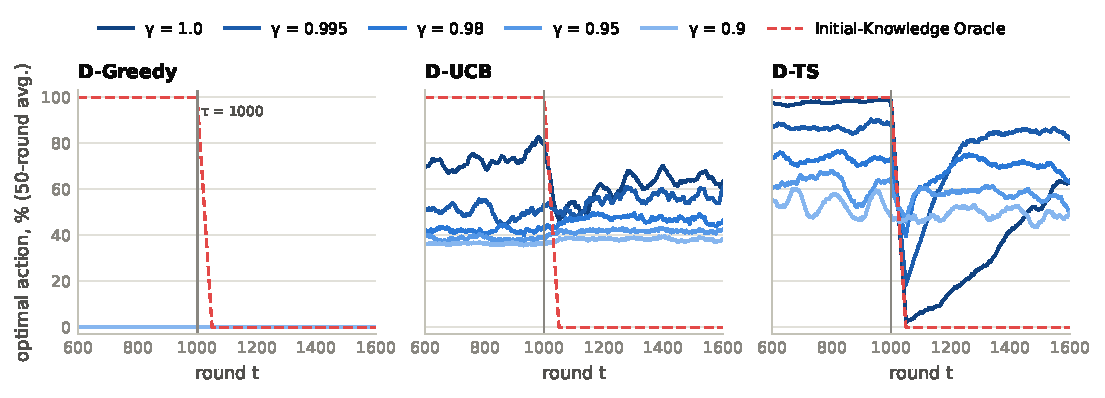
\includegraphics[width=0.92\linewidth]{fig3_e3_adaptation.pdf}
\caption{Single-agent E3: share of rounds in which the optimal action is chosen (50-round moving average) around the abrupt change at $\tau=1000$, for each discount factor. The initial-knowledge oracle keeps choosing the formerly best teammate.}\label{fig:e3}
\end{figure}

\subsection{E5: helpers learn when helping pays}
\Cref{fig:helping}(a) shows that the learned helpers' decisions depend on their own state. With MA-D-TS requesters, Q-learning helpers accept \ci{88.5}{2.0}\% of requests when idle, \ci{32.7}{9.6}\% at medium load, and \ci{25.7}{9.2}\% when busy; with MA-D-UCB the figures are 91.8\%, 48.3\% and 27.6\%. The informed threshold accepts 100\%, 79.3\% and 0\% in the same states. Learning therefore moves in the right direction but is too cautious at medium load and too willing when busy. Each helper is asked only about 450 times in 2000 rounds, spread over nine states, so value estimates for the rarely visited busy states remain noisy. The greedy helper policies are nevertheless stable: 99.1\% (MA-D-TS) and 99.4\% (MA-D-UCB) of well-visited states keep their greedy action between consecutive 50-round checkpoints.

\Cref{tab:e5} shows the cost of this imperfect learning and a real conflict of interest. Always-Accept gives requesters the most utility (0.603 with MA-D-TS), but helpers then also take tasks when busy. The informed threshold raises helper utility (0.136 vs.\ 0.123) and lowers requester utility (0.549). Q-learning helpers earn less than both (0.105, paired $p<10^{-8}$ for both comparisons with MA-D-TS). With MA-D-UCB requesters they match Always-Accept on helper utility (0.137 vs.\ 0.136, $p=0.44$) but stay below the informed rule (0.169, $p<10^{-6}$). When no one ever helps (Always-Reject), requesters fall below what working alone would give ($\Uself=0.35$), because their discounted beliefs do not become confident enough to stop them from asking. MA-Greedy never asks in any multi-agent setting: with uninformative priors its estimate $0.5\Uself+0.15$ lies below $\Uself$ for $\Uself>0.3$, so it never explores. It is therefore omitted from the tables.

\begin{table}[tbp]
\centering\footnotesize
\caption{E5: helper behaviour versus utility per round (mean\,$\pm$\,95\% CI, 30 seeds, $T=2000$). Accept\,\% is the share of received requests accepted. $^\dagger$Reference rule that knows its own $\theta_j$.}\label{tab:e5}
\begin{tabular}{llrrrrr}
\toprule
Helper policy & Requester & Accept\,\% & Ask\,\% & Requester util. & Helper util. & Welfare \\
\midrule
Always accept & MA-D-TS & 100.0 & 97.7{\scriptsize$\pm$0.2} & 0.603{\scriptsize$\pm$0.005} & 0.123{\scriptsize$\pm$0.002} & 0.727{\scriptsize$\pm$0.007} \\
 & MA-D-UCB & 100.0 & 100.0 & 0.559{\scriptsize$\pm$0.016} & 0.136{\scriptsize$\pm$0.021} & 0.696{\scriptsize$\pm$0.032} \\
\midrule
Always reject & MA-D-TS & 0.0 & 49.6{\scriptsize$\pm$0.2} & 0.300{\scriptsize$\pm$0.000} & 0.000 & 0.300{\scriptsize$\pm$0.000} \\
 & MA-D-UCB & 0.0 & 100.0 & 0.250 & 0.000 & 0.250 \\
\midrule
Informed threshold$^{\dagger}$ & MA-D-TS & 86.9{\scriptsize$\pm$0.5} & 96.2{\scriptsize$\pm$0.2} & 0.549{\scriptsize$\pm$0.004} & 0.136{\scriptsize$\pm$0.002} & 0.685{\scriptsize$\pm$0.007} \\
 & MA-D-UCB & 98.8{\scriptsize$\pm$0.4} & 100.0 & 0.565{\scriptsize$\pm$0.015} & 0.169{\scriptsize$\pm$0.008} & 0.734{\scriptsize$\pm$0.022} \\
\midrule
Q-learning (ours) & MA-D-TS & 69.0{\scriptsize$\pm$2.1} & 91.5{\scriptsize$\pm$0.9} & 0.479{\scriptsize$\pm$0.009} & 0.105{\scriptsize$\pm$0.004} & 0.584{\scriptsize$\pm$0.011} \\
 & MA-D-UCB & 82.1{\scriptsize$\pm$2.1} & 100.0 & 0.527{\scriptsize$\pm$0.010} & 0.137{\scriptsize$\pm$0.004} & 0.664{\scriptsize$\pm$0.012} \\
\bottomrule
\end{tabular}

\end{table}

\begin{figure}[tbp]
\centering
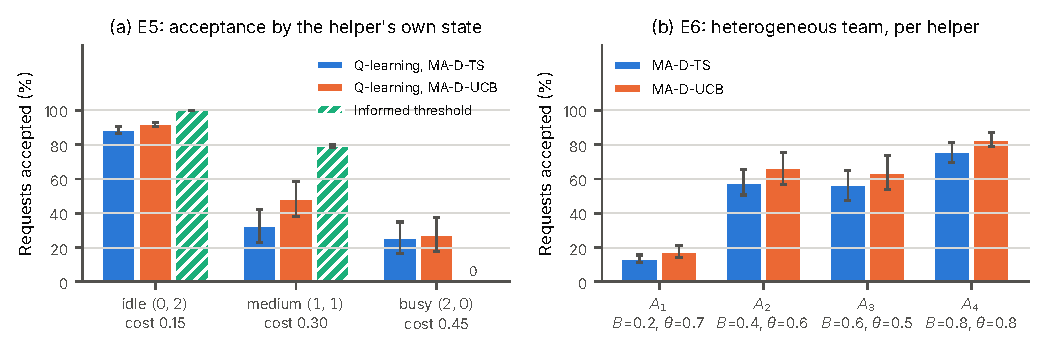
\includegraphics[width=\linewidth]{e5_e6_helping_behaviour.pdf}
\caption{(a) E5: share of requests accepted in the three diagonal helper states, by Q-learning helpers (two requester policies) and by the informed threshold. (b) E6: acceptance per agent in the heterogeneous team. Error bars: 95\% CI over 30 seeds.}\label{fig:helping}
\end{figure}

\subsection{E6: incentives shape who helps}
Varying the benefit $B$ of a successful help (\cref{tab:e6}) changes the team's behaviour, as each helper's own reward predicts. With $B=0.2$, accepting has negative expected payoff in almost every state, and helpers accept only \ci{9.5}{0.8}\% (MA-D-TS). With $B=0.8$, they accept \ci{82.1}{2.8}\%, and welfare rises from 0.309 to 0.800. In the heterogeneous team ($B=0.2,0.4,0.6,0.8$ for $A_1$--$A_4$; \cref{fig:helping}b), roles emerge without coordination. $A_4$, which is both the most willing and the most reliable, accepts 75.5\% of the requests it receives, is asked in 45.4\% of all rounds, and helps in 35.8\% of rounds. $A_1$ accepts 13.6\%, helps in only 1.3\% of rounds, and requesters learn to rarely ask it (9.3\% of rounds).

\begin{table}[tbp]
\centering\footnotesize
\caption{E6: effect of the helping benefit $B_j$ (mean\,$\pm$\,95\% CI, 30 seeds). Heterogeneous: $B=(0.2,0.4,0.6,0.8)$.}\label{tab:e6}
\begin{tabular}{lrrrrrr}
\toprule
 & \multicolumn{3}{c}{MA-D-TS} & \multicolumn{3}{c}{MA-D-UCB} \\
\cmidrule(lr){2-4}\cmidrule(lr){5-7}
Benefit $B_j$ & Accept\,\% & Requester util. & Welfare & Accept\,\% & Requester util. & Welfare \\
\midrule
$B=0.2$ & 9.5{\scriptsize$\pm$0.8} & 0.313{\scriptsize$\pm$0.002} & 0.309{\scriptsize$\pm$0.002} & 8.0{\scriptsize$\pm$0.6} & 0.278{\scriptsize$\pm$0.003} & 0.272{\scriptsize$\pm$0.003} \\
$B=0.5$ & 69.0{\scriptsize$\pm$2.1} & 0.479{\scriptsize$\pm$0.009} & 0.584{\scriptsize$\pm$0.011} & 82.1{\scriptsize$\pm$2.1} & 0.527{\scriptsize$\pm$0.010} & 0.664{\scriptsize$\pm$0.012} \\
$B=0.8$ & 82.1{\scriptsize$\pm$2.8} & 0.527{\scriptsize$\pm$0.013} & 0.800{\scriptsize$\pm$0.021} & 88.8{\scriptsize$\pm$1.0} & 0.539{\scriptsize$\pm$0.011} & 0.841{\scriptsize$\pm$0.015} \\
Heterogeneous & 64.4{\scriptsize$\pm$5.0} & 0.472{\scriptsize$\pm$0.022} & 0.607{\scriptsize$\pm$0.032} & 74.6{\scriptsize$\pm$4.3} & 0.499{\scriptsize$\pm$0.020} & 0.675{\scriptsize$\pm$0.026} \\
\bottomrule
\end{tabular}

\end{table}

\subsection{E7: changing teammate reliability}
At $t=1000$ the reliabilities change from $(0.9,0.7,0.6,0.5)$ to $(0.4,0.8,0.6,0.5)$: the best teammate becomes the worst, and another becomes the best ($\Uself=0.40$). Unlike the single-agent E3, the per-round discount $\gamma=0.98$ \emph{hurts} here: for MA-D-TS, total regret is 231.6 vs.\ 169.6 without discounting ($p<10^{-8}$), and post-change regret is 114.5 vs.\ 102.9 ($p=0.03$; \cref{tab:e7}, \cref{fig:e7}). The reason is that beliefs decay every global round, while each requester acts only every fourth round and splits its requests over three teammates. With $\gamma=0.98$ its memory of about 50 rounds holds only about four observations per teammate, so it keeps re-exploring. A discount of $\gamma=0.995$ gives each requester the same memory per own decision as $0.98$ in E3 ($0.995^4\approx0.98$). It lowers post-change regret for MA-D-UCB (83.3 vs.\ 98.6, $p=0.03$) and for MA-D-TS (93.9 vs.\ 102.9, $p=0.09$, not significant). It also raises pre-change regret (significantly for MA-D-TS: 85.1 vs.\ 66.7, $p=0.001$), so total regret is not significantly different from $\gamma=1$ ($p=0.17$ and $0.44$). Discounting must therefore be tuned to how often an agent sees each teammate, not to the global clock.

\begin{table}[tbp]
\centering\footnotesize
\caption{E7: abrupt reliability change at $t=1000$ (mean\,$\pm$\,95\% CI, 30 seeds, $T=2000$, Q-learning helpers).}\label{tab:e7}
\begin{tabular}{llrrrr}
\toprule
Requester & $\gamma$ & Pre-change regret & Post-change regret & Total regret & Post opt.\ action\,\% \\
\midrule
MA-D-TS & 1.00 & 66.7{\scriptsize$\pm$8.2} & 102.9{\scriptsize$\pm$10.3} & 169.6{\scriptsize$\pm$13.4} & 39.3{\scriptsize$\pm$3.8} \\
 & 0.995 & 85.1{\scriptsize$\pm$6.7} & 93.9{\scriptsize$\pm$5.7} & 178.9{\scriptsize$\pm$8.7} & 42.5{\scriptsize$\pm$2.7} \\
 & 0.98 & 117.0{\scriptsize$\pm$8.0} & 114.5{\scriptsize$\pm$5.1} & 231.6{\scriptsize$\pm$9.6} & 38.4{\scriptsize$\pm$1.9} \\
 & 0.95 & 154.3{\scriptsize$\pm$6.4} & 138.0{\scriptsize$\pm$3.0} & 292.2{\scriptsize$\pm$7.3} & 31.2{\scriptsize$\pm$0.8} \\
\midrule
MA-D-UCB & 1.00 & 76.0{\scriptsize$\pm$15.8} & 98.6{\scriptsize$\pm$12.4} & 174.5{\scriptsize$\pm$17.6} & 43.1{\scriptsize$\pm$6.5} \\
 & 0.995 & 82.9{\scriptsize$\pm$11.2} & 83.3{\scriptsize$\pm$10.0} & 166.2{\scriptsize$\pm$14.7} & 49.6{\scriptsize$\pm$6.0} \\
 & 0.98 & 110.0{\scriptsize$\pm$10.7} & 110.3{\scriptsize$\pm$6.5} & 220.3{\scriptsize$\pm$10.4} & 45.6{\scriptsize$\pm$3.8} \\
 & 0.95 & 135.7{\scriptsize$\pm$8.0} & 137.9{\scriptsize$\pm$5.8} & 273.6{\scriptsize$\pm$8.4} & 33.6{\scriptsize$\pm$2.3} \\
\bottomrule
\end{tabular}

\end{table}

\begin{figure}[tbp]
\centering
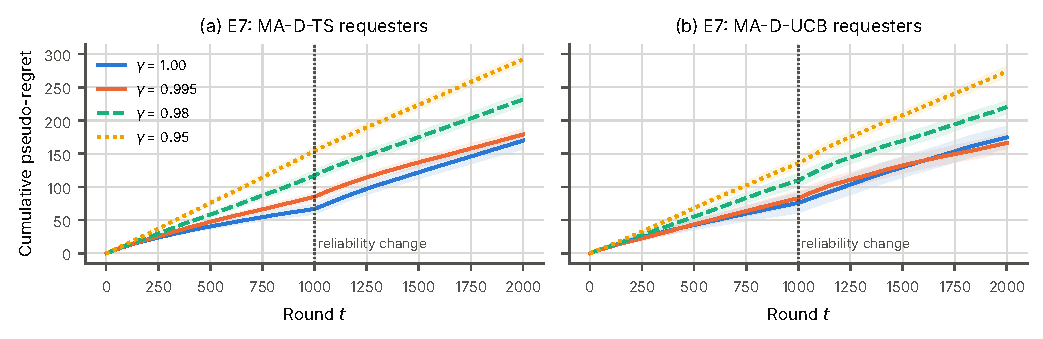
\includegraphics[width=\linewidth]{e7_changing_reliability.pdf}
\caption{E7: cumulative pseudo-regret for different discount factors (shaded: 95\% CI). Strong discounting raises regret both before and after the change.}\label{fig:e7}
\end{figure}

\subsection{E8: when to ask under deadlines}
\Cref{tab:e8} and \cref{fig:e8} compare the timing policies ($T=400$ tasks, reliability change at task 200). Working alone completes only \ci{40.3}{0.8}\% of tasks, so help matters. Learned timing completes \ci{55.1}{2.2}\% with requester reward \ci{0.199}{0.031}. It significantly outperforms Immediate evaluation (48.7\%, 0.087; $p=1.6\cdot10^{-4}$ and $p=4.4\cdot10^{-6}$) while sending 34.7\% fewer requests (62.3\% vs.\ 95.3\% of tasks), and it outperforms Never ask ($p<10^{-5}$). Immediate requests are also accepted less often (69.5\% vs.\ 81.4\% for Fixed delay), consistent with reaching teammates that are still busy from the previous task. Learned timing does \emph{not} beat the two hand-designed rules. Urgency (62.6\%, 0.297) and Fixed delay (61.4\%, 0.277) are significantly better ($p\le10^{-5}$ for completion and reward). A 27-state tabular policy trained on about 100 tasks per agent learns that waiting pays, but not exactly how long. This is not an artefact of exploration or short training: trained on 2000 tasks and then run greedily, it still completes only 55.1\% of the next 400 tasks, against 60.4\% for Urgency (\texttt{scripts/diagnose\_e8\_timing.py}). Planned timing, which computes the value of waiting from the learned beliefs, closes this gap: it completes \ci{60.5}{1.8}\% of tasks with requester reward \ci{0.288}{0.027}, significantly better than learned timing ($p<10^{-5}$), and its reward is not significantly different from Fixed delay ($p=0.18$) or Urgency ($p=0.28$). It sends far fewer requests (43.8\% of tasks vs.\ 79.0\% and 67.8\%, $p<10^{-5}$). Its completion rate is 2.0 points below Urgency ($p=0.002$), and team welfare is lower (0.349 vs.\ 0.398) because helpers, who earn from helping, are asked less. The timing policies are stable (93.4\% of well-visited states keep their greedy action over the last four 50-task checkpoints).

\begin{table}[tbp]
\centering\footnotesize
\caption{E8: timing policies under deadline $D=5$ (mean\,$\pm$\,95\% CI, 30 seeds, 400 tasks, MA-D-TS requesters, Q-learning helpers).}\label{tab:e8}
\begin{tabular}{lrrrrr}
\toprule
Timing policy & Completion\,\% & Ask\,\% & Solo attempts & Requester reward & Welfare \\
\midrule
Learned timing (Q-learning) & 55.1{\scriptsize$\pm$2.2} & 62.3{\scriptsize$\pm$4.5} & 3.63{\scriptsize$\pm$0.17} & 0.199{\scriptsize$\pm$0.031} & 0.279{\scriptsize$\pm$0.041} \\
Planned timing (model-based) & 60.5{\scriptsize$\pm$1.8} & 43.8{\scriptsize$\pm$1.3} & 4.39{\scriptsize$\pm$0.03} & 0.288{\scriptsize$\pm$0.027} & 0.349{\scriptsize$\pm$0.033} \\
Immediate evaluation & 48.7{\scriptsize$\pm$2.4} & 95.3{\scriptsize$\pm$0.6} & 2.45{\scriptsize$\pm$0.12} & 0.087{\scriptsize$\pm$0.038} & 0.185{\scriptsize$\pm$0.044} \\
Fixed delay ($k=2$) & 61.4{\scriptsize$\pm$2.2} & 79.0{\scriptsize$\pm$1.1} & 3.46{\scriptsize$\pm$0.06} & 0.277{\scriptsize$\pm$0.034} & 0.398{\scriptsize$\pm$0.042} \\
Urgency ($\tau_{\mathrm{rem}}\le 2$) & 62.6{\scriptsize$\pm$2.3} & 67.8{\scriptsize$\pm$1.0} & 4.02{\scriptsize$\pm$0.03} & 0.297{\scriptsize$\pm$0.034} & 0.398{\scriptsize$\pm$0.041} \\
Never ask & 40.3{\scriptsize$\pm$0.8} & 0.0 & 5.00{\scriptsize$\pm$0.00} & 0.024{\scriptsize$\pm$0.012} & 0.024{\scriptsize$\pm$0.012} \\
\bottomrule
\end{tabular}

\end{table}

\begin{figure}[tbp]
\centering
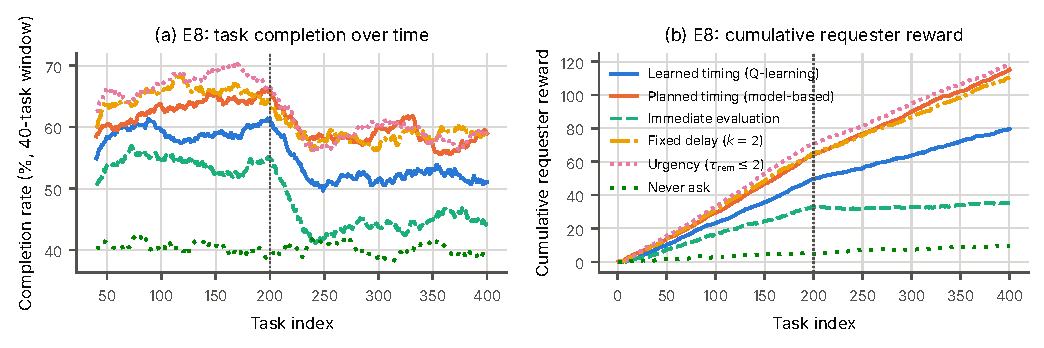
\includegraphics[width=\linewidth]{e8_temporal_help_seeking.pdf}
\caption{E8: (a) completion rate (40-task moving window) and (b) cumulative requester reward; dotted line: reliability change.}\label{fig:e8}
\end{figure}

\section{Discussion and limitations}\label{sec:discussion}
The system is multi-agent in a concrete sense. A helper's best action depends on its state; its state depends on how often requesters ask it; and requesters, who cannot see that state, experience it only as a changing acceptance probability. E5 and E6 show that agents adapt to this coupling (state-dependent acceptance, emergent specialisation), and E8 shows its effect on timing.

The results also show the limits of simple learners. Independent tabular Q-learning has no convergence guarantee among co-adapting agents~\cite{claus1998dynamics,hu2003nash}, and our helpers stay below an informed rule. A count-based learning rate and four times longer training narrow the gap but do not close it (helper utility 0.120 vs.\ 0.136 at $T=8000$; \texttt{scripts/diagnose\_e5\_helpers.py}): the informed rule knows its own reliability, which a learner must estimate from few, noisy outcomes per state. The policy-stability figures measure only that greedy actions stop changing, not that they are optimal. Requesters model each teammate's acceptance as a single rate, although it depends on the teammate's load; conditioning beliefs on observable signals (e.g.\ how recently a teammate helped) is a natural extension. Reliability does not depend on workload, help is one-to-one, and tasks arrive round-robin. Finally, model-free learned timing remains behind well-chosen heuristics; planning with the learned beliefs matches them, but it relies on knowing the solo-progress model and on a frozen-belief approximation.

\section{Group contributions}\label{sec:contributions}
\begin{itemize}[leftmargin=*]
  \item \textbf{Cherukuri Harshith Sai (24110091):} multi-agent architecture, temporal help-seeking model and timing Q-learning policy, dynamic oracle, report writing. \emph{Status: fulfilled.}
  \item \textbf{Atragada Venkata Naga Sai Ganesh (24110060):} multi-agent and temporal environments, agent state transitions and helping cost, state-visitation tracking, test suite (198 tests). \emph{Status: fulfilled.}
  \item \textbf{Ambati Chaitanya Ram (24110035):} helper Q-learning with decision-epoch updates, acceptance and reliability beliefs, experiments E5--E7 and result processing. \emph{Status: fulfilled.}
  \item \textbf{Dasari Lohith (24110100):} timing baselines, experiment E8, table and figure generation, dashboard integration. \emph{Status: fulfilled.}
\end{itemize}

\section{Code and reproducibility}\label{sec:repo}
Code, configurations, raw per-seed results, and the README with screenshots are at \url{https://github.com/HarshithSai91/Decentralized-MultiAgent-HelpSeeking}. Every table and figure in this report is produced from the raw results by \texttt{scripts/generate\_multiagent\_figures\_and\_tables.py} (E5--E8) and \texttt{scripts/analyze\_results.py} (E1--E4, S1--S5). The experiments are deterministic given the seed: rerunning \texttt{scripts/run\_all\_experiments.py} reproduces the raw results exactly.

\section{Conclusion}\label{sec:conclusion}
We turned a single-agent help-seeking bandit into a decentralized team in which every agent learns when, whether, and whom to ask, and whether to help. Making the cost of helping depend on the helper's own load gives helpers a real decision, which they learn to make, imperfectly, from individual rewards. Incentives decide who ends up helping. Belief discounting must match how often an agent observes each teammate. Learned timing improves on asking immediately but not on good heuristics, whereas planning with the learned beliefs matches the best heuristics with far fewer requests.

\bibliographystyle{plainnat}
\bibliography{references}

\end{document}
